

In computer graphics, 3D objects can often be parametrized by functions.
Moreover, low to medium accuracy interpolation is usually sufficient to project
satisfactory visual preceptions. In the following example, we use \funappxg to
interpolate the surface of a seashell, leading to a sufficiently accurate
three-dimensional reconstruction.

\begin{figure}[th]
  \centering
  \begin{tabular}{cc}
  \includegraphics[width=35mm]{figure/funappxseashell.eps} & \includegraphics[width=83mm]{figure/seashellsurferror.eps}\\
  a) & b)
  \end{tabular}
 \caption{a) Approximate seashell; b) Error estimation of seashell with tolerance $0.1$.}
  \label{fig:funappxseashell}
\end{figure}
\begin{exmp}
 
Figure~\ref{fig:funappxseashell}a) is an approximation of a pretty Florida
seashell, portrayed as a parametric surface in 3D. Let $a=-0.2$, $b=0.5$,
$c=0.1$, $n = 2$, $u,v \in [0, 2 \pi]$, and $w(v) =
a\left(1-\frac{v}{2\pi}\right)$. The parametric surface is defined by the
following equations in~\cite{DavEtal05}:
\begin{align*}
x(u,v) & =   \left[ w(v) \left(1+\cos(u)\right) + c\right]\cos(nv),\\
y(u,v) & = \left[w(v) (1+\cos(u)) + c\right] \sin(nv),\\
z(u,v) & = {bv}/{2\pi} + w(v)\sin(u).
\end{align*}
%
\begin{comment}
If a function of two variables $f(x,y)$ can be separated, such as
$$f(x,y)=f_1(x)+f_2(y) \text{ or } f(x,y)=f_1(x)f_2(y),$$ we can apply
\texttt{funappx\_g} directly to $f_1(x)$ and $f_2(y)$. However, $x(u,v)$,
$y(u,v)$, and $z(u,v)$ can not be represented by the form mentioned above.
Instead,
\end{comment}
%We approximate $\sin(x)$ and $\cos(x)$ on the interval $[0,4\pi]$. Denote
$sinappx(x)$ and $cosappx(x)$ as the approximate functions of $\sin(x)$ and
$\cos(x)$ on the interval $[0,4\pi]$, respectively; and let the resultant
approximants of $x(u,v)$, $y(u,v)$, and $z(u,v)$ as $\hat{x}(u,v)$,
$\hat{y}(u,v)$, and $\hat{z}(u,v)$, respectively.
\begin{comment}
Then we have
\begin{align*}
    \hat{x}(u,v) & =  \left[a\left(1-\frac{v}{2\pi}\right)\left(1+cosappx(u)\right) + c\right]cosappx(nv),\\
\hat{y}(u,v) & = \left[a\left(1-\frac{v}{2\pi}\right)(1+cosappx(u)) + c\right] sinappx(nv),\\
\hat{z}(u,v) & = \frac{bv}{2\pi} + a\left(1-\frac{v}{2\pi}\right)sinappx(u).
\end{align*}
\end{comment}
Define the overall error measure as
\begin{align*}
\mathscr{E} =  \max\limits_{u,v \in [0, 2 \pi] } & \left\{   |x(u,v)-\hat{x}(u,v)|,\right.
   \left.  |y(u,v)-\hat{y}(u,v)|, 
                                  \ \    |z(u,v)-\hat{z}(u,v)|\right\}.
\end{align*}
Even if we set the error tolerance as big as $0.1$, we still can obtain
Figure~\ref{fig:funappxseashell}a), which is very similar to the original
seashell image. The associated error plot is presented in
Figure~\ref{fig:funappxseashell}b), which shows that the approximation error
$\mathscr{E}=2 \times 10^{-4}$.
\end{exmp}

In digital animation, frames of images are produced to represent movements of
objects over small discrete time. To automatically insert frames between a
beginning frame and an ending frame, interpolation can be applied to estimating
the object's positions by using parametric curves that represent a trajectory in
3D as $(x(t), y(t), z(t))$, where each of the three coordinates in space is
parametrized by time $t$.  We refer readers to Example~5 in \cite{Din15a}, for instance.



\begin{exmp}
Chebfun is a MATLAB toolbox known for using Chebyshev polynomial basis for
approximating given functions to machine precision. In this example, we show
that it is challenged by $f_3$, defined in Section~\ref{sec:cone}. Around $x=0$
and $x=0.2$, the errors spike to more than $10^{-5}$. In contrast, the error of
the interpolant from \funappxg is uniformly below $10^{-14}$.

\begin{figure}[t]
\centering
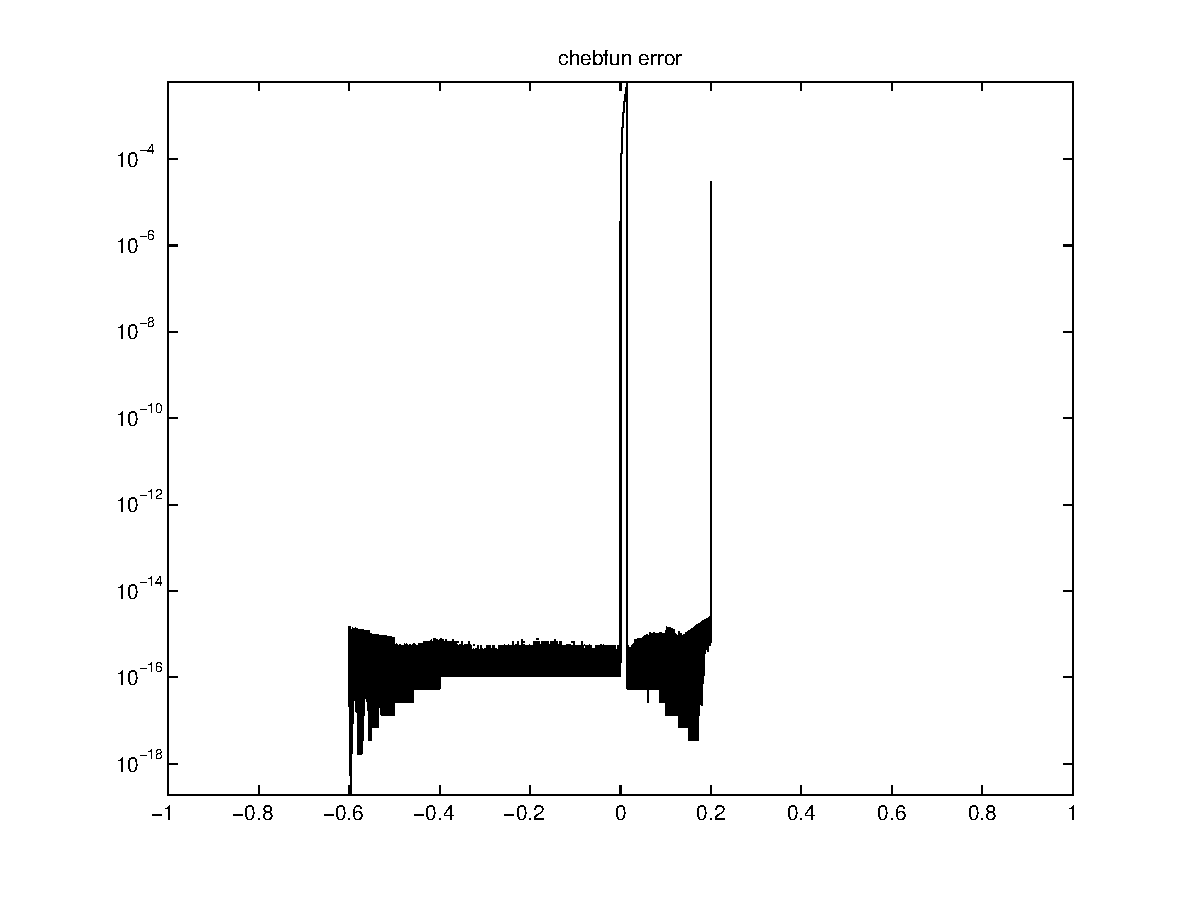
\includegraphics[width=6.2cm]{figure/chebfunf3.eps} \hspace{-5ex}
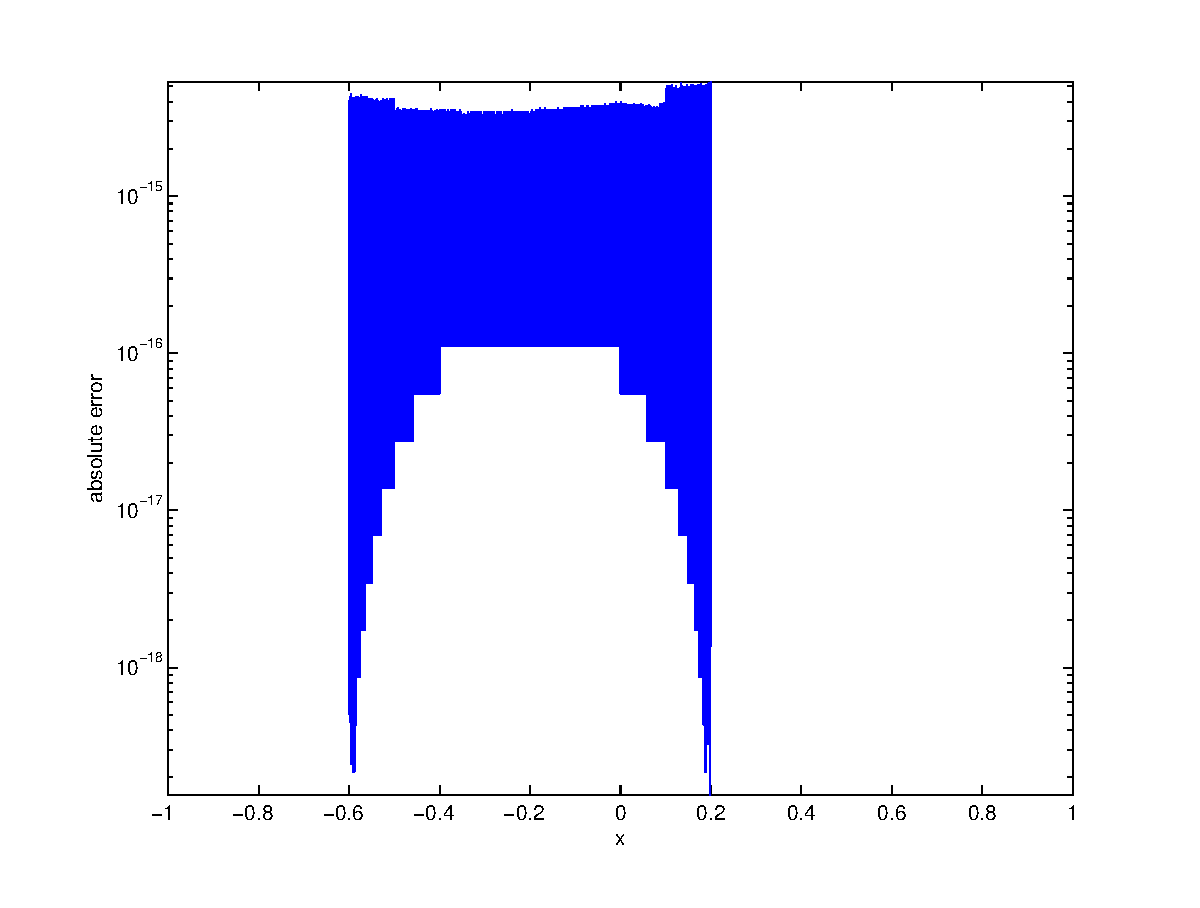
\includegraphics[width=6.2cm]{figure/funappxNoPenaltyf3.eps}
\caption{The example $f_3$ with errors of interpolants from chebfun (left) and \funappxg (right).}
\label{f3fig}
\end{figure}
\end{exmp}

\begin{comment}
Our algorithm is readily extensible to the following complex-valued function.
\begin{exmp}
This example is taken from MATLAB's documentation for \texttt{interp1}. 
Define the complex valued function
$v(x) = 5x + x^2 i$ for $x \in [1,10]$.  It is clear that the real part of $v$ 
is $5x$ and the imaginary part is $x^2$. We could  
apply \funappxg  to approximate the two parts separately. However, it is unnecessary.

\end{exmp}
\end{comment}

\begin{exmp}
In this example, we consider the function $f_4(x) = sin(10 \pi x^4) + x$, which is increasing oscillating over the interval $[0,2]$.
We use \funappxg, \funming, and \integralg to approximate the function, locate its global minimum, and estimate its integral with $\abstol = 10^{-8}$.
With $1,972,359$ points, \funappxg can approximate $f_4$ uniformly accurate as shown in Figure~\ref{f4fig}(a).
The true global minimum is $(0.6212340312, -0.3782149854)$ and the absolute approximation error of \funming using $n=2,022,621$ points is      
$(1.4\times 10^{-7}, 4.7\times 10^{-11})$. The integral 
$\int_{0}^{2} f_4 (x) dx = 2.145517314$ and the approximation error of \integralg is $4.7\times10^{-10}$ using $4,965,641$ points.

\begin{figure}[bt]
\centering
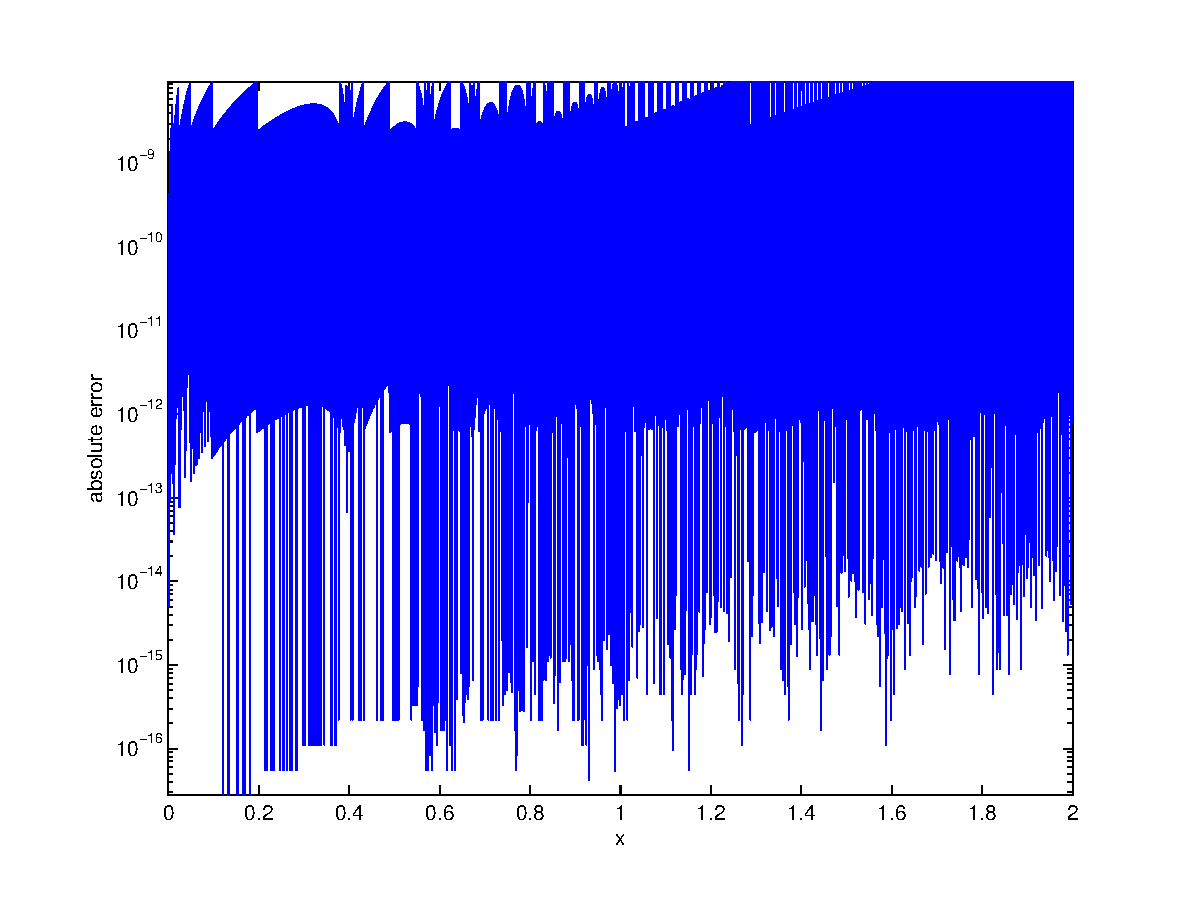
\includegraphics[width=6.2cm]{figure/f4_funappx_error.eps} \hspace{-5ex}
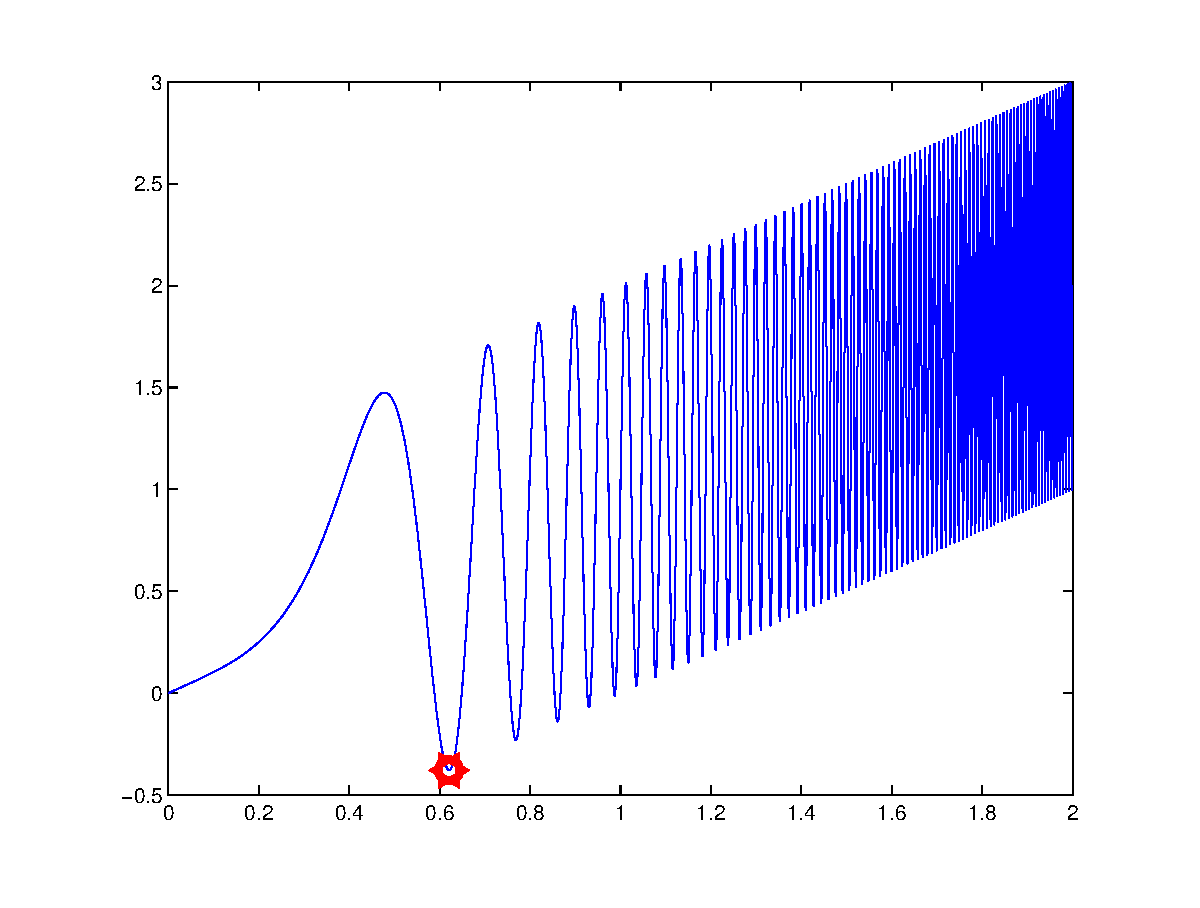
\includegraphics[width=6.2cm]{figure/f4_funmin_g.eps}
\caption{The example $f_4$ with errors of interpolants from \funappxg (left) and minimum found by \funming (right).}
\label{f4fig}
\end{figure}
\end{exmp}
